\documentclass[12pt,a4paper]{report}

% -------------------------------------------------
% PACOTES
% -------------------------------------------------
\usepackage[utf8]{inputenc}
\usepackage[T1]{fontenc}
\usepackage[brazil]{babel}
\usepackage{geometry}
\usepackage{graphicx}
\usepackage{float}
\usepackage{amsmath}
\usepackage{amssymb}
\usepackage{hyperref}
\usepackage{indentfirst}
\usepackage{setspace}
\usepackage{titlesec}
\usepackage{booktabs}
\usepackage{caption}
\usepackage{subcaption}
\usepackage{longtable}
\usepackage{array}
\usepackage{xcolor}
\usepackage{colortbl}
\usepackage{pdflscape}
\usepackage{pgfgantt}

% -------------------------------------------------
% CONFIGURAÇÕES GERAIS
% -------------------------------------------------
\geometry{
    a4paper,
    left=3cm,
    right=2cm,
    top=3cm,
    bottom=2cm
}

\onehalfspacing
\setlength{\parindent}{1.25cm}

\definecolor{ganttblue}{RGB}{52,100,145}
\definecolor{ganttgray}{RGB}{180,180,180}
\definecolor{ganttgreen}{RGB}{40,120,80}
\definecolor{ganttred}{RGB}{180,50,50}

% -------------------------------------------------
% DOCUMENTO
% -------------------------------------------------
\begin{document}

% -------------------------------------------------
% CAPA
% -------------------------------------------------
\begin{titlepage}
    \centering

    \textbf{ESEG -- Grupo ETAPA}\\
    \textbf{Engenharia da Computação}\\
    \vspace{3cm}

    \textbf{Ramon Vieira}\\
    \textbf{Nícolas Pereira}\\
    \textbf{Vinicius Venancio}\\
    \textbf{Kaique Rissato}\\

    \vfill

    \textbf{FACEGATEWAY: SISTEMA DE CONTROLE DE ENTRADA E SAÍDA BASEADO EM RECONHECIMENTO FACIAL}\\
    \vspace{0.5cm}
    Projeto de Sistema Embarcado com Processamento e Análise Logística

    \vfill

    SÃO PAULO\\
    2026

\end{titlepage}

% -------------------------------------------------
% FOLHA DE ROSTO
% -------------------------------------------------
\begin{titlepage}
    \centering

    \textbf{Ramon Vieira}\\
    \textbf{Nícolas Pereira}\\
    \textbf{Vinicius Venancio}\\
    \textbf{Kaique Rissato}\\

    \vspace{3cm}

    \textbf{FACEGATEWAY: SISTEMA DE CONTROLE DE ENTRADA E SAÍDA BASEADO EM RECONHECIMENTO FACIAL}

    \vspace{1.5cm}

    \begin{flushright}
        Trabalho apresentado ao Curso de Engenharia da\\
        Computação na ESEG como requisito parcial para\\
        obtenção da nota na disciplina Computação Embarcada.\\
        \vspace{0.5cm}
        Professor: Filippo Filho
    \end{flushright}

    \vfill

    SÃO PAULO\\
    2026

\end{titlepage}

% -------------------------------------------------
% ELEMENTOS PRÉ-TEXTUAIS
% -------------------------------------------------
\pagenumbering{roman}

\tableofcontents
\newpage

\listoffigures
\newpage

\listoftables
\newpage

% -------------------------------------------------
% INÍCIO DO TEXTO
% -------------------------------------------------
\pagenumbering{arabic}

% =================================================
\chapter{Introdução}
% =================================================

\section{Contextualização}

O controle de entrada e saída de funcionários é uma atividade essencial para organizações que operam com turnos fixos ou escalas de trabalho. Métodos tradicionais, como cartões magnéticos, senhas ou registros manuais, apresentam limitações relacionadas à segurança, possibilidade de fraudes e baixa integração com sistemas analíticos.

Com o avanço das técnicas de Visão Computacional e Aprendizado de Máquina, especialmente no campo do reconhecimento facial, tornou-se viável implementar soluções biométricas com processamento local e custo relativamente reduzido. Dispositivos embarcados de baixo consumo energético, como o Raspberry Pi 4, permitem a execução de modelos de aprendizado de máquina diretamente no ponto de captura, reduzindo latência e dependência de infraestrutura centralizada.

Além do controle de acesso, a coleta estruturada desses dados possibilita análises logísticas relevantes, como cálculo de tempo médio de permanência, identificação de padrões de atraso e avaliação de horários de entrada e saída. Essas informações podem apoiar decisões estratégicas relacionadas à gestão de recursos humanos.

\section{Problema de Pesquisa}

Como implementar um sistema de controle de acesso baseado em reconhecimento facial utilizando hardware de baixo custo, garantindo desempenho adequado, confiabilidade na identificação e geração de métricas logísticas úteis para análise organizacional, mantendo os dados biométricos restritos ao dispositivo embarcado?

\section{Objetivos}

\subsection{Objetivo Geral}

Desenvolver um sistema de controle de entrada e saída de funcionários baseado em reconhecimento facial, com processamento embarcado em C++ na Raspberry Pi 4 e backend analítico em Rust, expondo métricas logísticas via painel web e mobile.

\subsection{Objetivos Específicos}

\begin{itemize}
    \item Implementar pipeline de visão computacional em C++ capaz de detectar e reconhecer rostos em tempo real, com latência inferior a 500\,ms.
    \item Garantir operação offline completa -- catraca e buzzer funcionam independentemente de conectividade de rede.
    \item Transmitir eventos de acesso ao backend via protocolo MQTT com garantia de entrega (QoS\,1).
    \item Desenvolver API REST em Rust (Axum) com autenticação JWT e endpoints de analytics.
    \item Persistir embeddings e eventos no PostgreSQL com extensão pgvector para busca por similaridade.
    \item Desenvolver painel multiplataforma em Ionic + Angular, instalável como Progressive Web App.
    \item Estimar e documentar os custos de hardware necessários para implantação do MVP.
\end{itemize}

\section{Justificativa}

A adoção de sistemas biométricos no controle de acesso reduz vulnerabilidades associadas a métodos tradicionais, como empréstimo de cartões ou compartilhamento de credenciais. O reconhecimento facial elimina a necessidade de contato físico e integra-se de forma transparente ao fluxo de entrada e saída.

Do ponto de vista técnico, o projeto demonstra a viabilidade de execução de modelos de aprendizado de máquina em dispositivos embarcados de baixo custo, explorando otimização de desempenho com o formato ONNX e integração entre hardware e software em C++.

Uma decisão central de projeto é manter o reconhecimento facial completamente \textit{on-device}: nenhuma imagem bruta ou dado biométrico trafega pela rede. Apenas metadados de eventos (identificador do funcionário, horário, resultado) são enviados ao servidor, contribuindo diretamente para conformidade com princípios de minimização de dados da LGPD.

% =================================================
\chapter{Fundamentação Teórica}
% =================================================

\section{Reconhecimento Facial}

O reconhecimento facial é uma área da Visão Computacional dedicada à identificação ou verificação da identidade de um indivíduo a partir de características faciais extraídas de imagens ou vídeos. Sistemas modernos operam em três etapas principais: detecção facial, extração de características e comparação.

A detecção consiste na identificação da presença de um rosto em uma imagem. Neste projeto, utiliza-se o modelo \textbf{BlazeFace} (Google MediaPipe), exportado no formato ONNX, que além das \textit{bounding boxes} fornece \textit{keypoints} faciais -- posições dos olhos, nariz e boca -- essenciais para o alinhamento do rosto antes da geração do embedding.

A extração de características utiliza o modelo \textbf{MobileFaceNet}, treinado com a função de perda ArcFace no dataset MS-Celeb. O modelo gera embeddings de 128 dimensões que capturam as características discriminativas do rosto. A identificação ocorre pela comparação da distância de cosseno entre o embedding extraído e os embeddings previamente armazenados: valores abaixo de um limiar ($\approx 0{,}45$) indicam correspondência positiva.

\section{Edge Computing e Sistemas Embarcados}

O conceito de \textit{Edge Computing} destaca a importância do processamento local, reduzindo dependência de servidores remotos e minimizando latência. No caso de controle de acesso, o processamento embarcado permite resposta imediata à tentativa de autenticação, além de evitar a exposição de dados biométricos em redes externas.

A execução de modelos de aprendizado de máquina em hardware limitado é viabilizada pelo formato \textbf{ONNX} (\textit{Open Neural Network Exchange}), que permite exportar modelos treinados em qualquer framework e executá-los via \textbf{ONNXRuntime} com API C++, otimizando o uso de recursos disponíveis na Raspberry Pi 4.

\section{Protocolos de Comunicação IoT}

O protocolo \textbf{MQTT} (\textit{Message Queuing Telemetry Transport}) é o padrão de mercado para comunicação em dispositivos IoT. Seu modelo \textit{publish/subscribe} desacopla produtor e consumidor de mensagens, e os níveis de qualidade de serviço (QoS) garantem entrega mesmo em redes instáveis. No nível QoS\,1, o broker retém mensagens enquanto o subscriber estiver offline, garantindo que nenhum evento de acesso seja perdido.

\section{Aspectos Legais e Éticos}

Informações biométricas são classificadas como dados sensíveis pela Lei Geral de Proteção de Dados (LGPD -- Lei 13.709/2018), pois estão diretamente associadas à identidade do indivíduo. Entre os princípios aplicáveis ao projeto destacam-se:

\begin{itemize}
    \item Finalidade específica e legítima para coleta dos dados;
    \item Minimização: armazenamento de embeddings, não de imagens brutas;
    \item Transparência quanto ao uso das informações coletadas;
    \item Garantia de segurança e confidencialidade dos dados armazenados.
\end{itemize}

A decisão de manter o reconhecimento facial exclusivamente \textit{on-device} é diretamente motivada por esses princípios, eliminando o risco de vazamento de dados biométricos em trânsito.

% =================================================
\chapter{Arquitetura do Sistema}
% =================================================

\section{Visão Geral}

O sistema é organizado em três camadas físicas e lógicas independentes: o módulo embarcado (Raspberry Pi 4), o servidor local (notebook do desenvolvedor, substituível por nuvem em produção) e o painel web/mobile. A Figura~\ref{fig:arquitetura} apresenta o diagrama geral da arquitetura.

\begin{figure}[H]
    \centering
    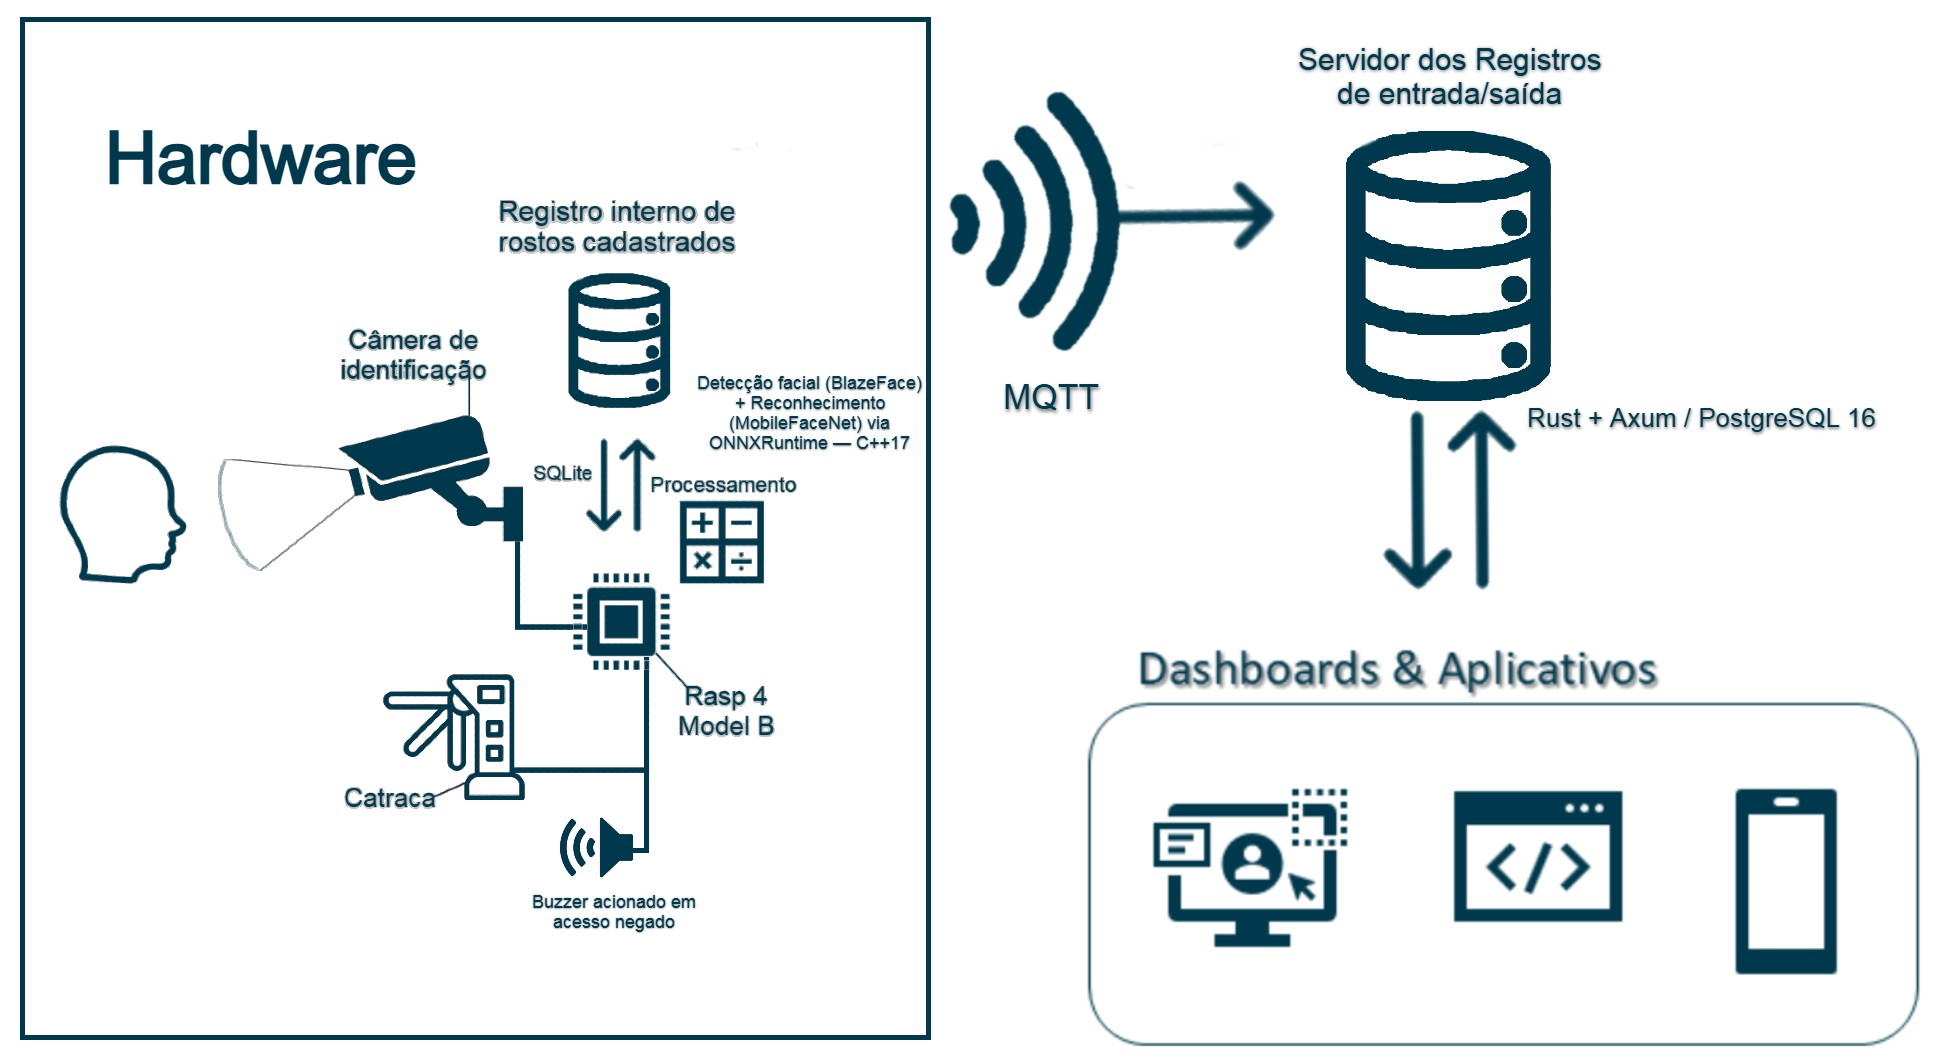
\includegraphics[width=0.92\textwidth]{arquitetura.png}
    \caption{Diagrama geral da arquitetura do FaceGateway}
    \label{fig:arquitetura}
\end{figure}

O fluxo operacional completo ocorre nas seguintes etapas:

\begin{enumerate}
    \item Câmera CSI captura frames continuamente.
    \item BlazeFace detecta presença de rosto e extrai \textit{keypoints} para alinhamento.
    \item MobileFaceNet gera embedding de 128 dimensões do rosto alinhado.
    \item Embedding é comparado por distância de cosseno com o cache local SQLite.
    \item Decisão: acesso concedido aciona relé da catraca via GPIO; acesso negado aciona buzzer.
    \item Evento é publicado no broker MQTT (tópico \texttt{facegate/events/access}).
    \item Subscriber Rust consome o evento e persiste no PostgreSQL.
    \item Painel Ionic + Angular consulta a API REST e exibe métricas ao gestor.
\end{enumerate}

O módulo embarcado opera de forma completamente autônoma: em caso de falha de rede, eventos são enfileirados em SQLite local e enviados ao broker quando a conectividade é restabelecida.

\section{Módulo Embarcado -- Raspberry Pi 4}

O módulo embarcado é responsável por toda a inteligência de visão computacional e atuação física. O hardware é composto por:

\begin{itemize}
    \item Raspberry Pi 4 Model B (4\,GB de RAM);
    \item Câmera CSI de 5 megapixels;
    \item Relé para acionamento da catraca (via GPIO);
    \item Buzzer para sinalização de acesso negado (via GPIO).
\end{itemize}

O software embarcado é desenvolvido em \textbf{C++17} e utiliza as seguintes bibliotecas:

\begin{itemize}
    \item \textbf{libcamera}: captura de frames via interface CSI;
    \item \textbf{OpenCV 4.8}: pré-processamento de imagem;
    \item \textbf{ONNXRuntime 1.17}: inferência dos modelos BlazeFace e MobileFaceNet;
    \item \textbf{Eigen3}: cálculo de distância de cosseno entre embeddings;
    \item \textbf{SQLite3}: cache local de embeddings e fila de eventos offline;
    \item \textbf{libmosquitto}: publicação de eventos no broker MQTT.
\end{itemize}

\section{Backend -- Servidor Local}

O backend é desenvolvido em \textbf{Rust} e composto pelos seguintes componentes:

\begin{itemize}
    \item \textbf{Axum 0.7}: framework HTTP para a API REST;
    \item \textbf{sqlx 0.7}: queries verificadas em \textit{compile-time} contra o PostgreSQL;
    \item \textbf{rumqttc 0.24}: subscriber MQTT assíncrono integrado ao runtime Tokio;
    \item \textbf{jsonwebtoken}: geração e validação de tokens JWT para autenticação do painel.
\end{itemize}

O banco de dados utilizado é o \textbf{PostgreSQL 16} com a extensão \textbf{pgvector 0.6}, que permite armazenar embeddings vetoriais e realizar busca por similaridade com índice HNSW diretamente no banco, eliminando a necessidade de biblioteca externa como FAISS.

A comunicação entre Raspberry e backend utiliza o protocolo \textbf{MQTT com QoS\,1}, com broker \textbf{Eclipse Mosquitto 2.x} rodando no servidor. A estrutura de tópicos é:

\begin{itemize}
    \item \texttt{facegate/events/access} -- evento de rosto reconhecido;
    \item \texttt{facegate/events/unknown} -- evento de rosto não reconhecido;
    \item \texttt{facegate/health} -- \textit{heartbeat} periódico do dispositivo.
\end{itemize}

\section{Painel Web e Mobile}

O painel é desenvolvido em \textbf{Ionic 7 + Angular 17}, gerando uma aplicação multiplataforma instalável como \textbf{Progressive Web App} (PWA) -- funciona no browser do desktop e pode ser instalado no celular como app nativo sem necessidade de loja de aplicativos.

As telas planejadas para o MVP são:

\begin{itemize}
    \item \textbf{Login}: autenticação JWT com \textit{guard} de rotas protegidas;
    \item \textbf{Dashboard}: cards de resumo e gráfico de fluxo de acessos por hora (ngx-echarts);
    \item \textbf{Funcionários}: listagem, cadastro e upload de foto para geração de embedding;
    \item \textbf{Histórico de eventos}: tabela paginada com filtros por funcionário e data;
    \item \textbf{Analytics}: atraso médio por funcionário e heatmap de presença por dia/hora.
\end{itemize}

% =================================================
\chapter{Organização do Projeto}
% =================================================

\section{Divisão de Tarefas}

O grupo é composto por quatro integrantes com as seguintes responsabilidades principais:

\begin{table}[H]
\centering
\caption{Divisão de responsabilidades por integrante}
\label{tab:divisao}
\begin{tabular}{>{\bfseries}p{2.8cm} p{3.5cm} p{7cm}}
\toprule
Integrante & Foco principal & Responsabilidades \\
\midrule
Ramon & Edge C++ + Rust crítico &
    Setup toolchain Raspberry, pipeline de visão (BlazeFace, MobileFaceNet, Eigen3),
    GPIO, autenticação JWT, sync de embeddings, ajuste de threshold \\
\addlinespace
Nícolas & Backend + banco &
    Setup PostgreSQL/pgvector, Mosquitto, subscriber MQTT,
    schema do banco, CRUD de funcionários, endpoints de analytics \\
\addlinespace
Kaique C & Suporte edge + integração &
    Buzzer GPIO, fila offline SQLite, apoio ao CRUD,
    tela de histórico de eventos, testes de integração, documentação \\
\addlinespace
Vinicius D & Frontend + design &
    Setup Ionic/Angular/PWA, tela de login, tela de funcionários,
    dashboard com gráficos, tela de analytics \\
\bottomrule
\end{tabular}
\end{table}

\section{Cronograma -- Diagrama de Gantt}

O semestre compreende 11 semanas de desenvolvimento entre a entrega do escopo (18/03) e a entrega final (27/05). O projeto possui três marcos intermediários definidos pelo professor, apresentados na Tabela~\ref{tab:marcos}.

\begin{table}[H]
\centering
\caption{Marcos do projeto}
\label{tab:marcos}
\begin{tabular}{lll}
\toprule
Data & Marco & Meta de conclusão \\
\midrule
18/03 & Entrega do escopo & Documento de arquitetura \\
22/04 & Entrega parcial 1 & $\approx$40\% -- Fases 1, 2 e 3 concluídas \\
13/05 & Entrega parcial 2 & $>$80\% -- Fases 4 e 5 concluídas \\
27/05 & Entrega final & Sistema integrado e documentado \\
03/06 & P2 & Avaliação individual \\
\bottomrule
\end{tabular}
\end{table}

O diagrama de Gantt a seguir apresenta a distribuição das atividades ao longo das semanas, com identificação das dependências entre tarefas e dos marcos de entrega.

% ---- GANTT 1: Fases 1-3 ----
% Largura útil landscape A4 com margens 3cm/2cm = 24.7cm
% Rótulos ocupam ~5.5cm → barras têm ~19.2cm para 6 colunas → x unit = 3.2cm
\begin{landscape}
\centering
\begin{ganttchart}[
    hgrid,
    vgrid={*{1}{dotted}},
    x unit=2cm,
    y unit title=0.65cm,
    y unit chart=0.65cm,
    title height=1,
    bar height=0.5,
    group right shift=0,
    group top shift=0.7,
    group height=.3,
    canvas/.append style={draw=black!20},
    bar/.append style={fill=ganttblue!70},
    group/.append style={fill=ganttgray!60, draw=black},
    milestone/.append style={fill=ganttred, draw=ganttred},
    title label font=\small,
    bar label font=\small,
    group label font=\small\bfseries,
    milestone label font=\small\bfseries,
    bar label node/.append style={text width=5cm, align=left},
    group label node/.append style={text width=5cm, align=left},
    milestone label node/.append style={text width=5cm, align=left}
]{1}{6}
 
\gantttitle{Fases 1--3: Infraestrutura, Visão e Atuação (18/mar -- 26/abr)}{6} \\
\gantttitle{S1 18/mar}{1}\gantttitle{S2 25/mar}{1}\gantttitle{S3 01/abr}{1}%
\gantttitle{S4 08/abr}{1}\gantttitle{S5 15/abr}{1}\gantttitle{S6 22/abr}{1} \\
 
\ganttgroup{Fase 1 -- Infraestrutura}{1}{3} \\
\ganttbar[bar/.append style={fill=ganttblue!60}]{1.1 Toolchain C++}{1}{2} \\
\ganttbar[bar/.append style={fill=ganttblue!60}]{1.2 PostgreSQL}{1}{1} \\
\ganttbar[bar/.append style={fill=ganttblue!60}]{1.3 Projeto Rust}{1}{2} \\
\ganttbar[bar/.append style={fill=ganttblue!60}]{1.4 Broker Mosquitto}{2}{2} \\
\ganttbar[bar/.append style={fill=ganttblue!60}]{1.5 Ionic + Angular + PWA}{1}{2} \\
\ganttbar[bar/.append style={fill=ganttblue!80}]{1.6 MQTT ponta a ponta}{3}{3} \\
 
\ganttgroup{Fase 2 -- Visão Comp}{2}{5} \\
\ganttbar[bar/.append style={fill=ganttgreen!60}]{2.1 Captura libcamera C++}{2}{2} \\
\ganttbar[bar/.append style={fill=ganttgreen!60}]{2.2 Detecção ONNX}{3}{3} \\
\ganttbar[bar/.append style={fill=ganttgreen!60}]{2.3 Alinhamento facial}{3}{4} \\
\ganttbar[bar/.append style={fill=ganttgreen!60}]{2.4 Embedding MobileFace}{4}{4} \\
\ganttbar[bar/.append style={fill=ganttgreen!80}]{2.5 Comparação + threshold}{4}{5} \\
\ganttbar[bar/.append style={fill=ganttgreen!60}]{2.6 CLI de enrollment SQLite}{5}{5} \\
 
\ganttgroup{Fase 3 -- Atuação Física}{5}{6} \\
\ganttbar[bar/.append style={fill=ganttgreen!70}]{3.1 GPIO catraca}{5}{5} \\
\ganttbar[bar/.append style={fill=ganttgreen!70}]{3.2 GPIO buzzer}{5}{5} \\
\ganttbar[bar/.append style={fill=ganttgreen!70}]{3.3 Fila offline SQLite}{6}{6} \\
 
\ganttmilestone{$\blacktriangledown$ Parcial 1 -- 40\%}{6}
 
\end{ganttchart}
\captionof{figure}{Gantt -- Fases 1 a 3: infraestrutura, visão computacional e atuação física (S1--S6)}
\label{fig:gantt1}
\end{landscape}
 
% ---- GANTT 2: Fases 4-6 ----
% 7 colunas → x unit = 19.2cm / 7 ≈ 2.7cm
\begin{landscape}
\centering
\begin{ganttchart}[
    hgrid,
    vgrid={*{1}{dotted}},
    x unit=2cm,
    y unit title=0.65cm,
    y unit chart=0.65cm,
    title height=1,
    bar height=0.5,
    group right shift=0,
    group top shift=0.7,
    group height=.3,
    canvas/.append style={draw=black!20},
    bar/.append style={fill=ganttblue!70},
    group/.append style={fill=ganttgray!60, draw=black},
    milestone/.append style={fill=ganttred, draw=ganttred},
    title label font=\small,
    bar label font=\small,
    group label font=\small\bfseries,
    milestone label font=\small\bfseries,
    bar label node/.append style={text width=5cm, align=left},
    group label node/.append style={text width=5cm, align=left},
    milestone label node/.append style={text width=5cm, align=left}
]{1}{7}
 
\gantttitle{Fases 4--6: Backend, Frontend e Entrega (15/abr -- 27/mai)}{7} \\
\gantttitle{S5 15/abr}{1}\gantttitle{S6 22/abr}{1}\gantttitle{S7 29/abr}{1}%
\gantttitle{S8 06/mai}{1}\gantttitle{S9 13/mai}{1}%
\gantttitle{S10 20/mai}{1}\gantttitle{S11 27/mai}{1} \\
 
\ganttgroup{Fase 4 -- Backend Rust}{1}{6} \\
\ganttbar[bar/.append style={fill=ganttblue!50}]{4.1 Schema banco}{1}{1} \\
\ganttbar[bar/.append style={fill=ganttblue!50}]{4.2 Subscriber MQTT}{2}{2} \\
\ganttbar[bar/.append style={fill=ganttblue!50}]{4.3 Auth JWT}{2}{3} \\
\ganttbar[bar/.append style={fill=ganttblue!50}]{4.4 CRUD funcionários}{3}{4} \\
\ganttbar[bar/.append style={fill=ganttblue!50}]{4.5 Sync embeddings Rasp}{4}{5} \\
\ganttbar[bar/.append style={fill=ganttblue!50}]{4.6 Endpoints de analytics}{5}{6} \\
 
\ganttgroup{Fase 5 -- Frontend Ionic}{3}{6} \\
\ganttbar[bar/.append style={fill=ganttblue!35}]{5.1 Tela de login JWT}{3}{4} \\
\ganttbar[bar/.append style={fill=ganttblue!35}]{5.2 Tela de funcionários}{4}{5} \\
\ganttbar[bar/.append style={fill=ganttblue!35}]{5.3 Histórico de eventos}{5}{6} \\
\ganttbar[bar/.append style={fill=ganttblue!35}]{5.4 Dashboard + gráficos}{6}{6} \\
\ganttbar[bar/.append style={fill=ganttblue!35}]{5.5 Analytics}{6}{6} \\
 
\ganttmilestone{$\blacktriangledown$ Parcial 2 -- 80\%}{6} \\
 
\ganttgroup{Fase 6 -- Integração}{6}{7} \\
\ganttbar[bar/.append style={fill=ganttgray!70}]{6.1 Sync edge $\leftrightarrow$ backend}{6}{6} \\
\ganttbar[bar/.append style={fill=ganttgray!70}]{6.2 Testes ponta a ponta}{6}{7} \\
\ganttbar[bar/.append style={fill=ganttgray!70}]{6.3 Ajuste de threshold}{7}{7} \\
\ganttbar[bar/.append style={fill=ganttgray!70}]{6.4 Documentação técnica}{7}{7} \\
\ganttbar[bar/.append style={fill=ganttgray!70}]{6.5 Preparação da demo}{7}{7} \\
 
\ganttmilestone{$\blacktriangledown$ Entrega Final}{7}
 
\end{ganttchart}
\captionof{figure}{Gantt -- Fases 4 a 6: backend, frontend e entrega final (S5--S11)}
\label{fig:gantt2}
\end{landscape}

\section{Estimativa de Custos}

A Tabela~\ref{tab:custos} apresenta os componentes de hardware necessários para o MVP, com preços estimados para o mercado brasileiro em 2026.

\begin{table}[H]
\centering
\caption{Estimativa de custo do hardware para o MVP}
\label{tab:custos}
\begin{tabular}{lrr}
\toprule
Componente & Quantidade & Preço estimado (R\$) \\
\midrule
Raspberry Pi 4 Model B -- 4\,GB & 1 & 650,00 \\
Câmera CSI 5MP (compatível RPi) & 1 & 120,00 \\
Cartão microSD 32\,GB (Class 10) & 1 & 40,00 \\
Fonte de alimentação USB-C 5V/3A & 1 & 50,00 \\
Módulo relé 5V (acionamento catraca) & 1 & 15,00 \\
Buzzer ativo 5V & 1 & 8,00 \\
Catraca de barreira (demonstração) & 1 & 180,00 \\
Jumpers e protoboard & 1 kit & 25,00 \\
\midrule
\textbf{Total estimado} & & \textbf{R\$ 1.088,00} \\
\bottomrule
\end{tabular}
\end{table}

Os custos de software são nulos: todas as tecnologias utilizadas -- Rust, C++, PostgreSQL, Mosquitto, Ionic, Angular e ONNXRuntime -- são de código aberto e gratuitas. O servidor local (notebook) já pertence ao grupo, eliminando custo de infraestrutura. Em um cenário de produção, o backend seria hospedado em nuvem, com custo variável conforme o provedor escolhido.

% =================================================
\chapter{Metodologia}
% =================================================

\section{Coleta de Dados e Cadastro de Funcionários}

O cadastro de um funcionário no sistema ocorre por meio de uma ferramenta de linha de comando (\textit{enrollment CLI}) desenvolvida em C++. O operador captura múltiplas fotos do funcionário em diferentes condições de iluminação e ângulo. Para cada imagem, o pipeline extrai o embedding via MobileFaceNet. O vetor resultante é armazenado na tabela \texttt{embeddings} do PostgreSQL, associado ao identificador do funcionário.

Nenhuma imagem bruta é persistida no banco de dados -- apenas os vetores de 128 dimensões. Isso atende diretamente ao princípio de minimização de dados da LGPD.

\section{Definição do Limiar de Autenticação}

O limiar de decisão (distância de cosseno) será ajustado empiricamente. Serão realizados testes comparando:

\begin{itemize}
    \item Embeddings do mesmo indivíduo em sessões distintas (testes positivos);
    \item Embeddings de indivíduos diferentes (testes negativos).
\end{itemize}

O objetivo é encontrar o valor que minimize simultaneamente a Taxa de Falsos Positivos (FAR -- \textit{False Accept Rate}) e a Taxa de Falsos Negativos (FRR -- \textit{False Reject Rate}). O valor inicial de referência é 0,45, com ajuste conforme os resultados dos testes.

\section{Testes e Avaliação}

A avaliação do sistema considerará:

\begin{itemize}
    \item \textbf{Precisão do reconhecimento}: acurácia, FAR e FRR com os rostos dos integrantes do grupo;
    \item \textbf{Latência}: tempo total desde a captura do frame até a decisão de acesso (meta: $<$500\,ms);
    \item \textbf{Resiliência offline}: eventos gerados sem rede são entregues ao broker ao reconectar;
    \item \textbf{Consistência das métricas}: valores de analytics verificados manualmente contra os registros brutos no banco.
\end{itemize}

% =================================================
\chapter{Desenvolvimento}
% =================================================

\section{Implementação do Sistema}

% A ser preenchido conforme o desenvolvimento avançar.

\section{Integração dos Módulos}

% A ser preenchido conforme o desenvolvimento avançar.

\section{Desafios Técnicos}

% A ser preenchido conforme o desenvolvimento avançar.

% =================================================
\chapter{Resultados}
% =================================================

\section{Desempenho do Modelo}

% A ser preenchido após os testes.

\section{Tempo de Processamento}

% A ser preenchido após os testes.

\section{Análise Logística Gerada}

% A ser preenchido após os testes.

% =================================================
\chapter{Discussão}
% =================================================

% A ser preenchido. Tópicos previstos:
% - Análise crítica dos resultados
% - Limitações do MVP (ambiente controlado, número reduzido de usuários)
% - Escalabilidade (múltiplas catracas, backend em nuvem)
% - Questões éticas e LGPD

% =================================================
\chapter{Conclusão}
% =================================================

% A ser preenchido. Tópicos previstos:
% - Retomada dos objetivos
% - Contribuições do projeto
% - Trabalhos futuros (Jetson Nano, OAuth2 corporativo, múltiplos dispositivos)

% =================================================
\chapter*{Referências}
\addcontentsline{toc}{chapter}{Referências}
% =================================================

\begin{itemize}
    \item DENG, J. et al. \textbf{ArcFace: Additive Angular Margin Loss for Deep Face Recognition}. CVPR, 2019.
    \item BAZAREVSKY, V. et al. \textbf{BlazeFace: Sub-millisecond Neural Face Detection on Mobile GPUs}. Google Research, 2019.
    \item CHEN, S. et al. \textbf{MobileFaceNets: Efficient CNNs for Accurate Real-Time Face Verification on Mobile Devices}. CCBR, 2018.
    \item MICROSOFT. \textbf{ONNX Runtime: Cross-platform inference accelerator}. Disponível em: \url{https://onnxruntime.ai}. Acesso em: mar. 2026.
    \item ECLIPSE FOUNDATION. \textbf{Eclipse Mosquitto: An open source MQTT broker}. Disponível em: \url{https://mosquitto.org}. Acesso em: mar. 2026.
    \item PGVECTOR. \textbf{Open-source vector similarity search for Postgres}. Disponível em: \url{https://github.com/pgvector/pgvector}. Acesso em: mar. 2026.
    \item BRASIL. \textbf{Lei n.\ 13.709, de 14 de agosto de 2018}. Lei Geral de Proteção de Dados Pessoais (LGPD). Brasília, DF, 2018.
\end{itemize}

% =================================================
\appendix

\chapter{Especificações Técnicas}

\begin{table}[H]
\centering
\caption{Stack tecnológico completo}
\label{tab:stack}
\begin{tabular}{llll}
\toprule
Camada & Tecnologia & Versão & Função \\
\midrule
Edge -- linguagem & C++17 & GCC 12+ & Pipeline de visão e GPIO \\
Edge -- visão & OpenCV & 4.8 & Captura e pré-processamento \\
Edge -- inferência & ONNXRuntime & 1.17 & Execução dos modelos ONNX \\
Edge -- álgebra & Eigen3 & 3.4 & Distância de cosseno \\
Edge -- cache & SQLite & 3.x & Embeddings e fila offline \\
Edge -- MQTT & libmosquitto & 2.x & Publicação de eventos \\
Broker & Eclipse Mosquitto & 2.x & Roteamento MQTT \\
Backend & Rust + Axum & 1.78 / 0.7 & API REST \\
Backend -- banco & sqlx & 0.7 & Queries compile-time \\
Backend -- MQTT & rumqttc & 0.24 & Subscriber assíncrono \\
Backend -- auth & jsonwebtoken & 9.x & JWT HS256 \\
Banco de dados & PostgreSQL + pgvector & 16 / 0.6 & Persistência + busca vetorial \\
Frontend & Ionic + Angular & 7 / 17 & Painel web/mobile PWA \\
Frontend -- gráficos & ngx-echarts & 17.x & Visualizações de analytics \\
\bottomrule
\end{tabular}
\end{table}

\chapter{Trechos Relevantes de Código}

% A ser preenchido conforme a implementação avançar.

\end{document}
